%
\documentclass[12pt]{article}
\usepackage{mathtools}
\usepackage{amsmath}
%\usepackage[fleqn]{amsmath}
\usepackage{amsthm}
\usepackage{mathrsfs}
\usepackage{amssymb}
\usepackage{amsfonts}
\usepackage{multicol}
\usepackage{fancyhdr}
\usepackage{graphicx}
%\usepackage{subfigure}
\usepackage{subfig} % to include multiple figures
\usepackage[usenames]{color}
\usepackage[skip=5pt]{caption} % for figure captions
\usepackage{float} % to use [H] for figures
\usepackage{listings}
\usepackage{verbatim}

% \usepackage[final,notref,notcite,color]{showkeys}
\usepackage[left=1in,top=1in,right=1in,bottom=1in,letterpaper]{geometry}
\renewcommand{\baselinestretch}{1.2}

\pagestyle{fancy}
\lhead{}
\chead{}
\rhead{}
\lfoot{}
\cfoot{\thepage}
\rfoot{}


% \usepackage{subfigure}

\renewcommand{\headrulewidth}{0.4pt}
\renewcommand{\footrulewidth}{0.4pt}
\renewcommand{\lim}{\mathrm{lim}}

\renewcommand{\ln}{\mathrm{ln}}



%\usepackage{versions}
%\includeversion{prop}
%    \excludeversion{prop}
%    \includeversion{dem}

%\mathtoolsset{showonlyrefs}

%% macros for editing and commenting
\usepackage[normalem]{ulem} % to use \sout
\newcommand{\remove}[1]{{\color{Gray}\sout{#1}}}
\newcommand{\revise}[1]{{\color{blue}#1}}
\newcommand{\comm}[1]{{\color{red}(yx: #1)}}

\newcommand{\bm}[1]{\boldsymbol{#1}}


%% macros for vectors
\newcommand{\va}{{\mathbf{a}}}
\newcommand{\vb}{{\mathbf{b}}}
\newcommand{\vc}{{\mathbf{c}}}
\newcommand{\vd}{{\mathbf{d}}}
\newcommand{\ve}{{\mathbf{e}}}
\newcommand{\vf}{{\mathbf{f}}}
\newcommand{\vg}{{\mathbf{g}}}
\newcommand{\vh}{{\mathbf{h}}}
\newcommand{\vi}{{\mathbf{i}}}
\newcommand{\vj}{{\mathbf{j}}}
\newcommand{\vk}{{\mathbf{k}}}
\newcommand{\vl}{{\mathbf{l}}}
\newcommand{\vm}{{\mathbf{m}}}
\newcommand{\vn}{{\mathbf{n}}}
\newcommand{\vo}{{\mathbf{o}}}
\newcommand{\vp}{{\mathbf{p}}}
\newcommand{\vq}{{\mathbf{q}}}
\newcommand{\vr}{{\mathbf{r}}}
\newcommand{\vs}{{\mathbf{s}}}
\newcommand{\vt}{{\mathbf{t}}}
\newcommand{\vu}{{\mathbf{u}}}
\newcommand{\vv}{{\mathbf{v}}}
\newcommand{\vw}{{\mathbf{w}}}
\newcommand{\vx}{{\mathbf{x}}}
\newcommand{\vy}{{\mathbf{y}}}
\newcommand{\vz}{{\mathbf{z}}}

%% macros for matrices
\newcommand{\vA}{{\mathbf{A}}}
\newcommand{\vB}{{\mathbf{B}}}
\newcommand{\vC}{{\mathbf{C}}}
\newcommand{\vD}{{\mathbf{D}}}
\newcommand{\vE}{{\mathbf{E}}}
\newcommand{\vF}{{\mathbf{F}}}
\newcommand{\vG}{{\mathbf{G}}}
\newcommand{\vH}{{\mathbf{H}}}
\newcommand{\vI}{{\mathbf{I}}}
\newcommand{\vJ}{{\mathbf{J}}}
\newcommand{\vK}{{\mathbf{K}}}
\newcommand{\vL}{{\mathbf{L}}}
\newcommand{\vM}{{\mathbf{M}}}
\newcommand{\vN}{{\mathbf{N}}}
\newcommand{\vO}{{\mathbf{O}}}
\newcommand{\vP}{{\mathbf{P}}}
\newcommand{\vQ}{{\mathbf{Q}}}
\newcommand{\vR}{{\mathbf{R}}}
\newcommand{\vS}{{\mathbf{S}}}
\newcommand{\vT}{{\mathbf{T}}}
\newcommand{\vU}{{\mathbf{U}}}
\newcommand{\vV}{{\mathbf{V}}}
\newcommand{\vW}{{\mathbf{W}}}
\newcommand{\vX}{{\mathbf{X}}}
\newcommand{\vY}{{\mathbf{Y}}}
\newcommand{\vZ}{{\mathbf{Z}}}

\newcommand{\vlam}{{\bm{\lambda}}}
\newcommand{\vtheta}{{\bm{\theta}}}
\newcommand{\veta}{{\bm{\eta}}}
\newcommand{\vell}{{\bm{\ell}}}
\newcommand{\vxi}{{\bm{\xi}}}


%% macros for sets
\newcommand{\cA}{{\mathcal{A}}}
\newcommand{\cB}{{\mathcal{B}}}
\newcommand{\cC}{{\mathcal{C}}}
\newcommand{\cD}{{\mathcal{D}}}
\newcommand{\cE}{{\mathcal{E}}}
\newcommand{\cF}{{\mathcal{F}}}
\newcommand{\cG}{{\mathcal{G}}}
\newcommand{\cH}{{\mathcal{H}}}
\newcommand{\cI}{{\mathcal{I}}}
\newcommand{\cJ}{{\mathcal{J}}}
\newcommand{\cK}{{\mathcal{K}}}
\newcommand{\cL}{{\mathcal{L}}}
\newcommand{\cM}{{\mathcal{M}}}
\newcommand{\cN}{{\mathcal{N}}}
\newcommand{\cO}{{\mathcal{O}}}
\newcommand{\cP}{{\mathcal{P}}}
\newcommand{\cQ}{{\mathcal{Q}}}
\newcommand{\cR}{{\mathcal{R}}}
\newcommand{\cS}{{\mathcal{S}}}
\newcommand{\cT}{{\mathcal{T}}}
\newcommand{\cU}{{\mathcal{U}}}
\newcommand{\cV}{{\mathcal{V}}}
\newcommand{\cW}{{\mathcal{W}}}
\newcommand{\cX}{{\mathcal{X}}}
\newcommand{\cY}{{\mathcal{Y}}}
\newcommand{\cZ}{{\mathcal{Z}}}


%
\newcommand{\vareps}{\varepsilon}

%% macros for the real and imaginary parts
\newcommand{\ri}{{\mathrm{i}}}
\newcommand{\rr}{{\mathrm{r}}}

%% macros for math notions and operators
\newcommand{\EE}{\mathbb{E}} % expectation
\newcommand{\RR}{\mathbb{R}} % real
\newcommand{\CC}{\mathbb{C}} % complex
\newcommand{\ZZ}{\mathbb{Z}} % integer
\renewcommand{\SS}{{\mathbb{S}}} % symmetric matrix
\newcommand{\SSp}{\mathbb{S}_{+}} % symmetric positive semi-definite matrix
\newcommand{\SSpp}{\mathbb{S}_{++}} % symmetric positive definite matrix
\newcommand{\sign}{\mathrm{sign}} % sign function
\newcommand{\vzero}{\mathbf{0}} % 0 vector
\newcommand{\vone}{{\mathbf{1}}} % 1 vector

\newcommand{\dist}{\mathrm{dist}}    % distance
\newcommand{\op}{{\mathrm{op}}} % subscript for operator norm
\newcommand{\opt}{{\mathrm{opt}}} % subscript for optimal solution
%\newcommand{\supp}{{\mathrm{supp}}} % support
\newcommand{\Prob}{{\mathrm{Prob}}} % probability
\newcommand{\prox}{{\mathbf{prox}}} % proximal map
\newcommand{\Diag}{{\mathrm{Diag}}} % vector -> diagonal matrix
\newcommand{\diag}{{\mathrm{diag}}} % matrix diagonal -> vector
\newcommand{\dom}{{\mathrm{dom}}} % domain
\newcommand{\rank}{\textnormal{rank}}
%\newcommand{\grad}{{\nabla}}    % gradient
\newcommand{\tr}{{\mathrm{tr}}} % trace
\newcommand{\TV}{{\mathrm{TV}}} % total variation
\newcommand{\Proj}{{\mathrm{Proj}}} % projection
\newcommand{\Null}{{\mathrm{Null}}} % null space
\newcommand{\Dim}{{\mathrm{dim}}} % dimension
\newcommand{\conv}{{\mathrm{conv}}} % convex hull
\newcommand{\clos}{{\mathrm{cl}}} % closure
\newcommand{\inte}{{\mathrm{int}}} % interior
\newcommand{\etal}{{\textit{et al.}}}
\newcommand{\conj}{{\mathrm{conj}}} % conjugate
\newcommand{\vvec}{{\mathrm{vec}}}
\newcommand{\fold}{{\mathbf{fold}}} % fold into a tensor
\newcommand{\unfold}{{\mathbf{unfold}}} % unfold a tensor
\newcommand{\fit}{{\mathrm{fit}}} % data fitting
\newcommand{\obj}{{\mathrm{obj}}} % data fitting
\newcommand{\round}{{\mathrm{round}}}
\newcommand{\epi}{\mathrm{epi}} %epigraph
\newcommand{\hyp}{\mathrm{hyp}} %hypograph

% rounding number
\newcommand{\err}{{\mathrm{err}}}
\newcommand{\ST}{\mbox{ subject to }}
\newcommand{\st}{\mbox{ s.t. }}

\newcommand{\ip}[2]{\langle #1 , #2 \rangle}
\newcommand{\by}{{\bf y}}
\newcommand{\bxs}{{\bf x}_{\epsilon,\lambda,q}}
\newcommand{\od}{\frac{d}{dt}}
\newcommand{\pd}{{\partial }}
\newcommand{\rankk}{{\hbox{rank}}}




\newcommand{\prev}{{\mathrm{prev}}} % previous iteration

\DeclareMathOperator{\shrink}{shrink} % shrinkage
\DeclareMathOperator{\hardthr}{hardthr} % hard thresholding
\DeclareMathOperator*{\argmin}{arg\,min} % argmin
\DeclareMathOperator*{\argmax}{arg\,max} % argmax

\DeclareMathOperator*{\Min}{minimize}
\DeclareMathOperator*{\Max}{maximize}



%% macros for environments math equations

\newcommand{\bc}{\begin{center}}
\newcommand{\ec}{\end{center}}

\newcommand{\bdm}{\begin{displaymath}}
\newcommand{\edm}{\end{displaymath}}

\newcommand{\beq}{\begin{equation}}
\newcommand{\eeq}{\end{equation}}

\newcommand{\bfl}{\begin{flushleft}}
\newcommand{\efl}{\end{flushleft}}

\newcommand{\bt}{\begin{tabbing}}
\newcommand{\et}{\end{tabbing}}

\newcommand{\beqn}{\begin{eqnarray}}
\newcommand{\eeqn}{\end{eqnarray}}

\newcommand{\beqs}{\begin{align*}} % no equation numbers
\newcommand{\eeqs}{\end{align*}}  % no equation numbers

%% macros for theorem-like environments

\newtheorem{theorem}{Theorem}[section]
%\newtheorem{acknowledgement}{Acknowledgement}[section]
%\newtheorem{axiom}{Axiom}[section]
%\newtheorem{algorithm}{Algorithm}[section]
%\newtheorem{case}{Case}[section]
\newtheorem{claim}{Claim}[section]
%\newtheorem{conclusion}{Conclusion}[section]
%\newtheorem{condition}{Condition}[section]
%\newtheorem{conjecture}{Conjecture}[section]
\newtheorem{corollary}{Corollary}[section]
%\newtheorem{criterion}{Criterion}[section]
\newtheorem{definition}{Definition}[section]
\newtheorem{example}{Example}[section]
%\newtheorem{exercise}{Exercise}[section]
\newtheorem{lemma}{Lemma}[section]
%\newtheorem{notation}{Notation}[section]
%\newtheorem{problem}{Problem}[section]
\newtheorem{proposition}{Proposition}[section]
\newtheorem{remark}{Remark}[section]
\newtheorem{assumption}{Assumption}
%\newtheorem{solution}{Solution}[section]
%\newtheorem{summary}{Summary}[section]



\newcommand{\hvx}{{\hat{\vx}}}
\DeclarePairedDelimiter{\dotp}{\langle}{\rangle} 
%% editing
\usepackage[shortlabels]{enumitem}
\usepackage[normalem]{ulem}
%\newcommand{\remove}[1]{{\color{Gray}\sout{#1}}}
%\newcommand{\comm}[1]{{\color{red}(#1)}}
%\newcommand{\revise}[1]{{\color{blue}#1}}


\title{Final Project (Robust PCA) - MATP 4820 }
\author{Thomas Shweh - Eric Tran}
\date{}

%%%%%%%%%%%%%%%%%
%
%  Listings colors
%
%%%%%%%%%%%%%%%%%

\definecolor{mygreen}{RGB}{28,172,0} % color values Red, Green, Blue
\definecolor{mylilas}{RGB}{170,55,241}

%%%%%%%%%%%%%%%%%
%
%  BEGIN DOCUMENT
%
%%%%%%%%%%%%%%%%%

\begin{document}

%%%%%%%%%%%%%%%%%
%
%  Listings preferences
%
%%%%%%%%%%%%%%%%%

\lstset{language=Matlab,%
    basicstyle=\footnotesize\ttfamily,
    breaklines=true,%
    morekeywords={matlab2tikz},
    deletekeywords={diff},
    keywordstyle=\color{blue},%
    %otherkeywords={self},             % Add keywords here
    identifierstyle=\color{black},%
    stringstyle=\color{mylilas},
    commentstyle=\color{mygreen},%
    showstringspaces=false,%without this there will be a symbol in the places where there is a space
    numbers=left,%
    numberstyle={\tiny \color{black}},% size of the numbers
    numbersep=9pt, % this defines how far the numbers are from the text
    %emph=[1]{for,end,break},emphstyle=[1]\color{red}, %some words to emphasise
    %emph=[2]{word1,word2}, emphstyle=[2]{style},    
}

%%%%%%%%%%%%%%%%%%%%%%%%%%%%%%
%
%  Make Title
%  Yes
%%%%%%%%%%%%%%%%%%%%%%%%%%%%%%

\maketitle
\noindent\textbf{Collaboration}\\
Thomas Shweh (shweht - 661774756): Quadratic Penalty, Graphs, Write up
\\
Eric Tran (trane2 - 661646071): Quadratic Penalty, ADMM, Write up 
\section*{Quadratic Penalty Method}
Given the constrained problem, we decided to implement a quadratic penalty method. Penalty methods replace a constrained optimization problem by a series of unconstrained problems; for this reason we decided to separate our original model into two subproblems for each update: $\vL$ and $\vS$.
\noindent
\newline
\textbf{Subproblems}
\newline
\noindent We can model the Robust PCA problem in the form
$$\min_{\vL, \vS}\|\vL\|_* + \lambda \|\vS\|_1 \qquad \text{s.t. }\vL + \vS = \vX$$
We can develop and iteration of the problem in form of an accelerated proximal gradient of this problem. Hence we will need to solve subproblems in the form
$$\min_{\vL, \vS}\|\vL\|_* + \lambda \|\vS\|_1  + \frac{\beta}{2}\|\vL + \vS - \vZ\|^2_F$$
Where $\beta$ is the penalty parameter. But we are going to express the equation in terms of $\mu$, a value that we were are going to use every iteration to accelerate the convergence. Thus our problem becomes
$$\min_{\vL, \vS}\mu\|\vL\|_* + \mu\lambda \|\vS\|_1  + \frac{1}{2}\|\vL + \vS - \vZ\|^2_F$$
With $\vX = (\vL, \vS)$, we can separate the function into two components $h(\vX) = \mu\|\vL\|_* + \mu\lambda \|\vS\|_1$ and $g(\vX) = \frac{1}{2}\|\vL + \vS - \vZ\|^2_F$. Since the nuclear norm is non differentiable we will work with the gradient of $g$ because it is differentiable. So $\nabla g(\vX) = (\nabla_\vL g(\vX), \nabla_\vS g(\vX))$ where $\nabla_\vL g(\vX) = \nabla_\vS g(\vX) = \vL + \vS - \vZ$.
Now finding the Lipshitz constant we have 
\begin{align*}
    \|\nabla g(\vX_1) - \nabla g(\vX_1) \| &= \left\|\begin{bmatrix}\vL_1 + \vS_1 - \vZ\\ \vL_1 + \vS_1 - \vZ\end{bmatrix} - \begin{bmatrix}\vL_2 + \vS_2 - \vZ\\ \vL_2 + \vS_2 - \vZ\end{bmatrix}\right\| \\
    &= \left\|\begin{bmatrix}\vL_1 - \vL_2 + \vS_1 - \vS_2\\ \vL_1 - \vL_2 + \vS_1 - \vS_2\end{bmatrix} \right\|\\
    &\leq \left\| \begin{bmatrix}\vL_1 - \vL_2\\\vS_1 - \vS_2 \end{bmatrix}\right\| + \left\| \begin{bmatrix}\vS_1 - \vS_2\\\vL_1 - \vL_2 \end{bmatrix}\right\|\\
    &= 2\|\vX_1 - \vX_2 \|
\end{align*}
Which leaves us with a Lipschitz constant of 2. Now we can express each iteration in the general form of the proximal gradient. This form is
$$x^+ = \argmin_u \left( h(u) + \frac{L}{2}\|u-G(y)\|^2\right)$$
So since each iteration we are updating $\vL, \vS$ together we have
\begin{align*}
    \vL_{k+1}, \vS_{k+1} &= \argmin_\vX \left(h(\vX) + \frac{L}{2}\| \vX - G(Y_k)\|^2 \right)\\
    &= \argmin_{\vL, \vS} \left(\mu \|L\|_* + \mu\lambda\|\vS\|_1 + \left\|\begin{bmatrix}\vL\\\vS\end{bmatrix} - \begin{bmatrix}G^\vL_k\\G^\vS_k\end{bmatrix} \right\|^2\right)\\
    &= \argmin_{\vL, \vS} \left(\|L\|_* + \frac{1}{2\frac{\mu}{2}}\|\vL - G^\vL_k\|^2 + \mu\lambda\|\vS\|_1 + \frac{1}{2\frac{\mu}{2}}\|\vS - G^\vS_k\|^2\right)
\end{align*}
Since the problem above is separable, we now have 2 problems that we can solve for. Essentially we can express the problems of finding $\vL_{k+1}, \vS_{k+1}$ in terms of the shrinkage operator. For $G^\vL_k = U\Sigma V^T$ or the SVD, we can express each iteration as such
\begin{align*}
    \vL_{k+1} &= U\mathcal{S}_{\frac{\mu}{2}}[\Sigma]V^T\\
    \vS_{k+1} &= \mathcal{S}_{\frac{\lambda\mu}{2}}[G^\vS_k]
\end{align*}
Our penalty term for our problem is, where $\bar{\mu}$ is the floor value for $\mu$.
$$\frac{1}{2\bar{\mu}} \|\vL + \vS - \vZ\|_F^2$$
\textbf{Shrinkage Operator}\\
The shrinkage operator is derived from the soft-thresholding rule found from Theorem 2.1 (referred to in the assignment/from LMS) which shows:
\begin{center}
    $\mathcal{S}_{\tau \lambda} = \argmin_{x} \dfrac{1}{2 \tau}||X - Y||^2_F + \lambda ||X||_1$
\end{center}
Because this expressions is convex, we understand that there is a unique minimizer, X, that can be found element-wise. Because of this we know that $Y_{r,c} - X_{r, c} \in \tau \lambda \partial|X_{r, c}|$ where $r, c$ indicates the element. From here, we can reason upon inspection that when $X_{r, c} = 0 \rightarrow |Y_{r,c}| \leq \lambda$ and $X_{r, c} \neq 0 \rightarrow \partial |X_{r, c}|$. This yields:
\begin{center}
    $X_{r, c} = Y_{r, c} - \tau \lambda sign(Y_{r, c}) = \mathcal{S}_{\tau}$
\end{center}
This is a summary of how we derived the shrinkage operator based on the paper from LMS (suggested in the assignment - Theorem 2.1) and our additional research (see references). This will be used for our proximal mapping.

\noindent \textbf{Stopping Condition}

\noindent We can derive the stopping conditions based off of the KKT conditions of the original problem. This will give us the primal and dual feasibility. The original KKT conditions of the problem are
$$\vL + \vS - \vZ = 0 \qquad Y^* \in \partial \|L\|_* \qquad Y^* \in \partial\|\lambda S\|_1$$
Thus the primal feasbility is the violation on the constraint on the problem. We will measure this error to be 
$$\|\vZ - \vL - \vS\|_F / \|\vZ\|_F$$
and we will terminate once we are within a certain tolerance. From our extensive testing we found that $1e^{-4}$ was a good tolerance to terminate for this condition.


\noindent Our second stopping condition happens when we have a violation of dual feasibility. This is measured by the expression
$$\dist (\partial \|L\|_*, \partial\|\lambda S\|_1) / \|\vZ\|_F$$
Where the distance is $\min \{\|x - y\|_F | x \in \partial \|L\|_*, y \in \partial\|\lambda S\|_1\}$.
However computing this distance is expensive because of the projection onto $\partial \|L\|_*$. So instead we will be using an approximation of $\mu_{k-1}\|S_k - S_{k-1}\|_F$. Thus our second stopping condition is 
$$\min(\mu_k, \sqrt{\mu_k}) \|S_k - S_{k-1}\|_F / \|\vZ\|_F$$
We have found that $1e^-6$ is a good tolerance to stop for this measure of error.\\

\noindent Our last stopping condition involves with the parameter $\mu$. For every iteration we decrease $\mu$ by a factor of $0.9$. This helps with convergence and allows us to terminate our loop at a point with accurate results. However, once we will terminate the loop if it appears problem will not converge. This is if $\mu$ reaches the floor $\bar{\mu}$, which we set at the value of $10^{-9} \times \mu_0$.
\newpage


\section*{Alternating Direction Method of Multipliers}
To minimize the problem using an ADMM, we will use the augmented Lagrangian which takes this form in its most general case:
\begin{center}
    $\mathcal{L} (L, S, Y, \mu) = f(x)_0 + \langle f(x), Y \rangle + \frac{\mu}{2}||f(x)||^2$
\end{center}
\newline
\textbf{Subproblems}
\newline
Applying this general case to our minimization problem where the two subproblems will be iteratively solving $\vS$ and $\vL$ such that $\vX = \vL + \vS$ yields the partial augmented Lagrangian:
\begin{center}
    $\mathcal{L} (L, S, Y, \mu) = ||L||_* + \lambda ||S||_1 + \langle X - L - S, Y \rangle + \frac{\mu}{2}||X - L - S||^2_F$
\end{center}
Rather than iteratively solving $\vL$ and $\vS$ separately at each step, the ADMM will alternately solve $\vL$ and $\vS$ where $\vS$ will be fixed to solve $\vL$ and $\vL$ will be fixed to solve $\vS$. We will find these updates by taking the minimum of the Lagrangian with respect to $\vL$ and $\vS$ such that:
\begin{center}
    $(L_{k+1}, S_{k+1}) = \argmin_{L, S} ||L||_* + \lambda ||S||_1 + \langle X - L - S, Y \rangle + \frac{\mu}{2}||X - L - S||^2_F$
\end{center}
By deriving each component, we yield $L_{k+1}$ and $S_{k+1}$:
\begin{center}
     $(L_{k+1}) = \argmin_{L} ||L||_* + \lambda ||S||_1 + \langle X - L - S, Y \rangle + \frac{\mu}{2}||X - L - S||^2_F$
     \newline
     $= \argmin_{L} ||L||_* + \dfrac{1}{2 \mu_k^{-1}} ||L - (X - S + \mu_k^{-1} Y)||^2_F$
     \newline
     $(S_{k+1}) = \argmin_{S} ||L||_* + \lambda ||S||_1 + \langle X - L - S, Y \rangle + \frac{\mu}{2}||X - L - S||^2_F$
     \newline
     $= \argmin_{S} \lambda ||S||_1 + \dfrac{1}{2 \mu_k^{-1}} ||S - (X - L + \mu_k^{-1} Y)||^2_F$
     \newline
\end{center}
Recognizing the form of these equations, recall the shrinkage operator (derived by the Theorem 2.1 of the paper from LMS) from the Quadratic Penalty Method above, such that we that apply the shrinkage operator to represent $L_{k+1}$ and $S_{k+1}$ in closed form. This will yield minimizers in the same form that we found in the Quadratic Penalty Method such that we are able to map the non-differentiable terms:
\begin{center}
    $L_{k+1} = U\mathcal{S}_{\mu_k^{-1}}[\Sigma]V^\top$
    \newline
    $S_{k+1} = \mathcal{S}_{\mu_k^{-1}}[X - L_{k+1} + \mu_k^{-1} Y]$
    \newline
\end{center}
Note the application of the shrinkage operator here is with the assumption that $U \Sigma V^\top = X - S + \mu_k^{-1} Y$ for the derivation of $L_{k+1}$. These closed-form solutions are our subproblems for our algorithm. Refer to shrinkage operator from Quadratic Penalty Method (as they are derived from the same logic).
\newline
\textbf{Iterative Update}
\newline
In addition to updating out subproblems, in each iteration we update $Y_{k+1}$ with the addition of the primal feasibility multiplied by a factor of the penalty parameter ($\mu$) such that $Y_{k+1} = Y + \mu (X - L - S)$. The penalty parameter is derived from the size of the data set and then scaled by 10. We chose this as our penalty parameter as we wanted the variable to fit relative to the data and multiplying it by a factor of 10 allowed our results to be clean. This provided the best results after extensive testing.
\newline
\textbf{Stopping Condition}
\newline
Our stopping condition is similar to the one we used in our Quadratic Penalty Method which defined the condition as $\dfrac{||X - L - S||_F}{||X||_F} < tol$ where $tol$ is a tolerance defined as $1.0e-4$. Refer to first stopping condition from Quadratic Penalty Method (as they are derived from the same logic).
\newpage


\section*{Comparison of Algorithms}
To run our code, be sure that the sample data, admm\_solver.m,  penalty\_solver.m, and test\_model\_RPCA.m scripts are in the same directory and run test\_model\_RPCA.m. This will call both scripts for both provided datasets (random data and escalator). Below is a sample output:
\\
\textbf{Output}\\ \\

\begin{minipage}{0.5\textwidth}
 \begin{verbatim}
ADMM Solver:
Random Data Test
||L-Lopt||/||Lopt|| = 3.2518e-05
||S-Sopt||/||Sopt|| = 9.6964e-04
Elapsed Time: 0.989668 seconds
Iterations: 13
Final residual: 9.5248e-05
--------------------
Escalator Data Test
See Output Images
Elapsed Time: 65.793886 seconds
Iterations: 220
Final residual: 9.9682e-05
 \end{verbatim}
\end{minipage}
\begin{minipage}{0.5\textwidth}
 \begin{verbatim}
Penalty Solver:
Random Data Test
||L-Lopt||/||Lopt|| = 4.6753e-05
||S-Sopt||/||Sopt|| = 8.9496e-04
Elapsed Time: 6.650571 seconds
Iterations: 99
Final residual: 9.3958e-05
--------------------
Escalator Data Test
See Output Images
Elapsed Time: 27.844079 seconds
Iterations: 113
Final residual: 9.3651e-05
 \end{verbatim}
\end{minipage}
\newpage
\begin{figure}[H]%
   \centering
   \subfloat[L3 ADMM]{{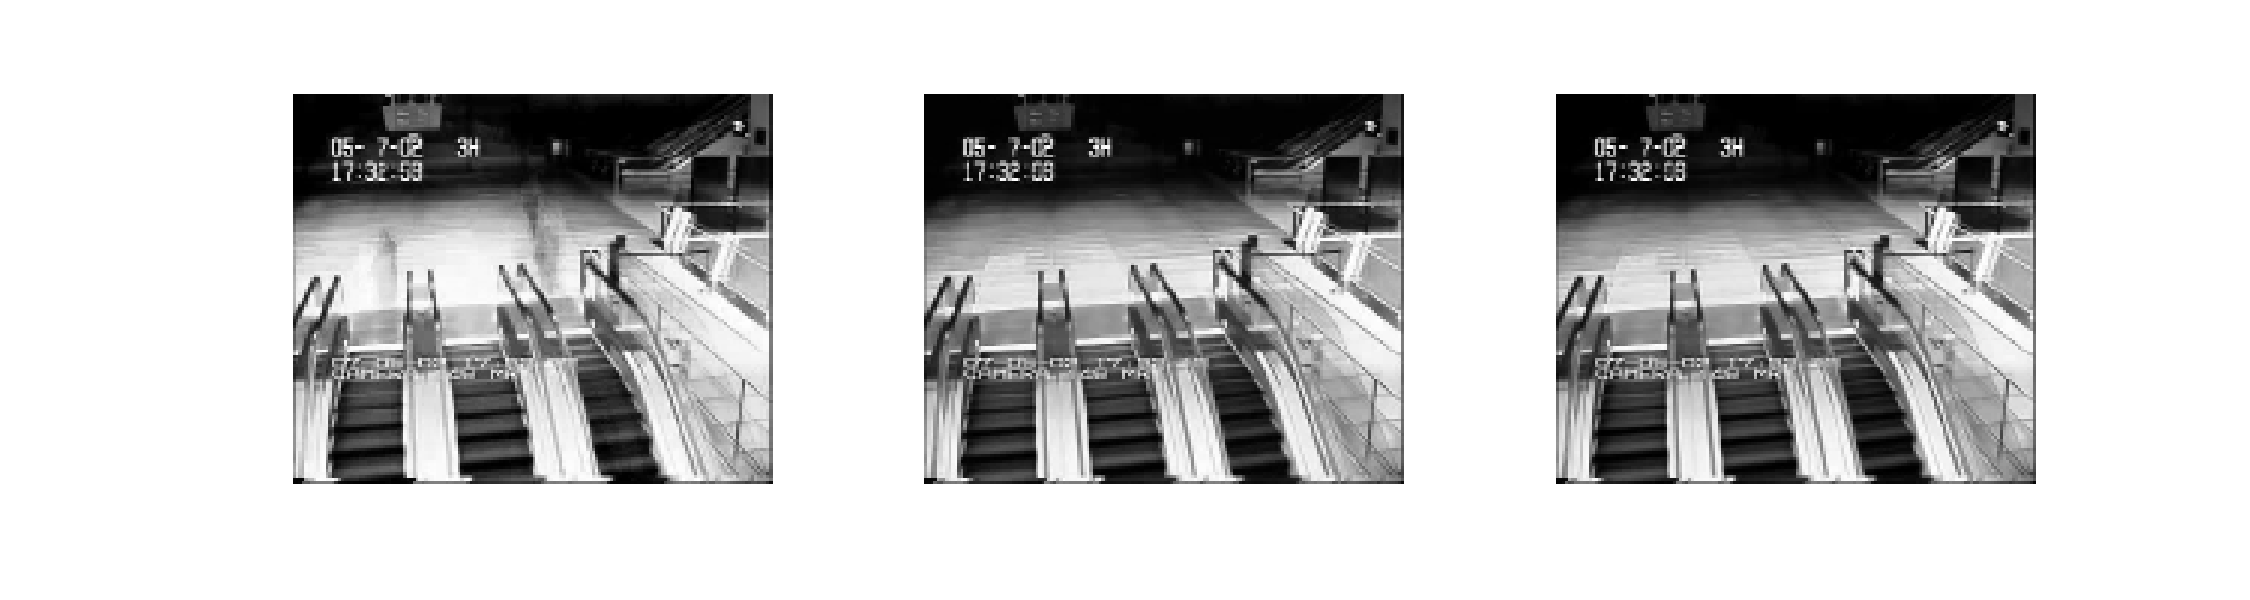
\includegraphics[width=6in]{L3slices_ADMM.pdf} }}%
   \\
   \subfloat[S3 ADMM]{{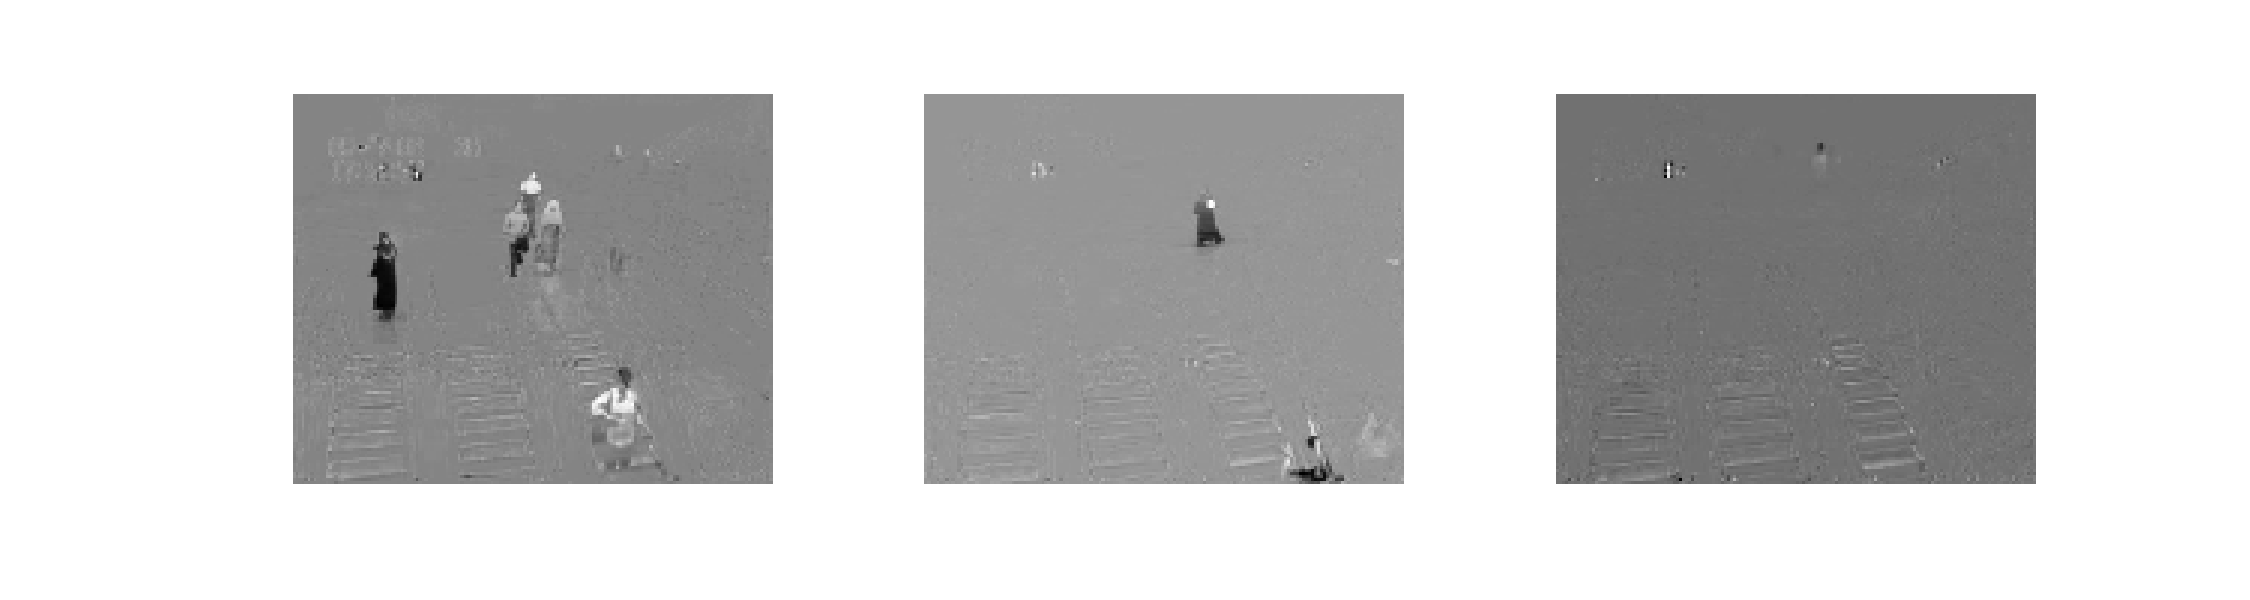
\includegraphics[width=6in]{S3slices_ADMM.pdf} }}%
   \\
    \subfloat[L3 Penalty]{{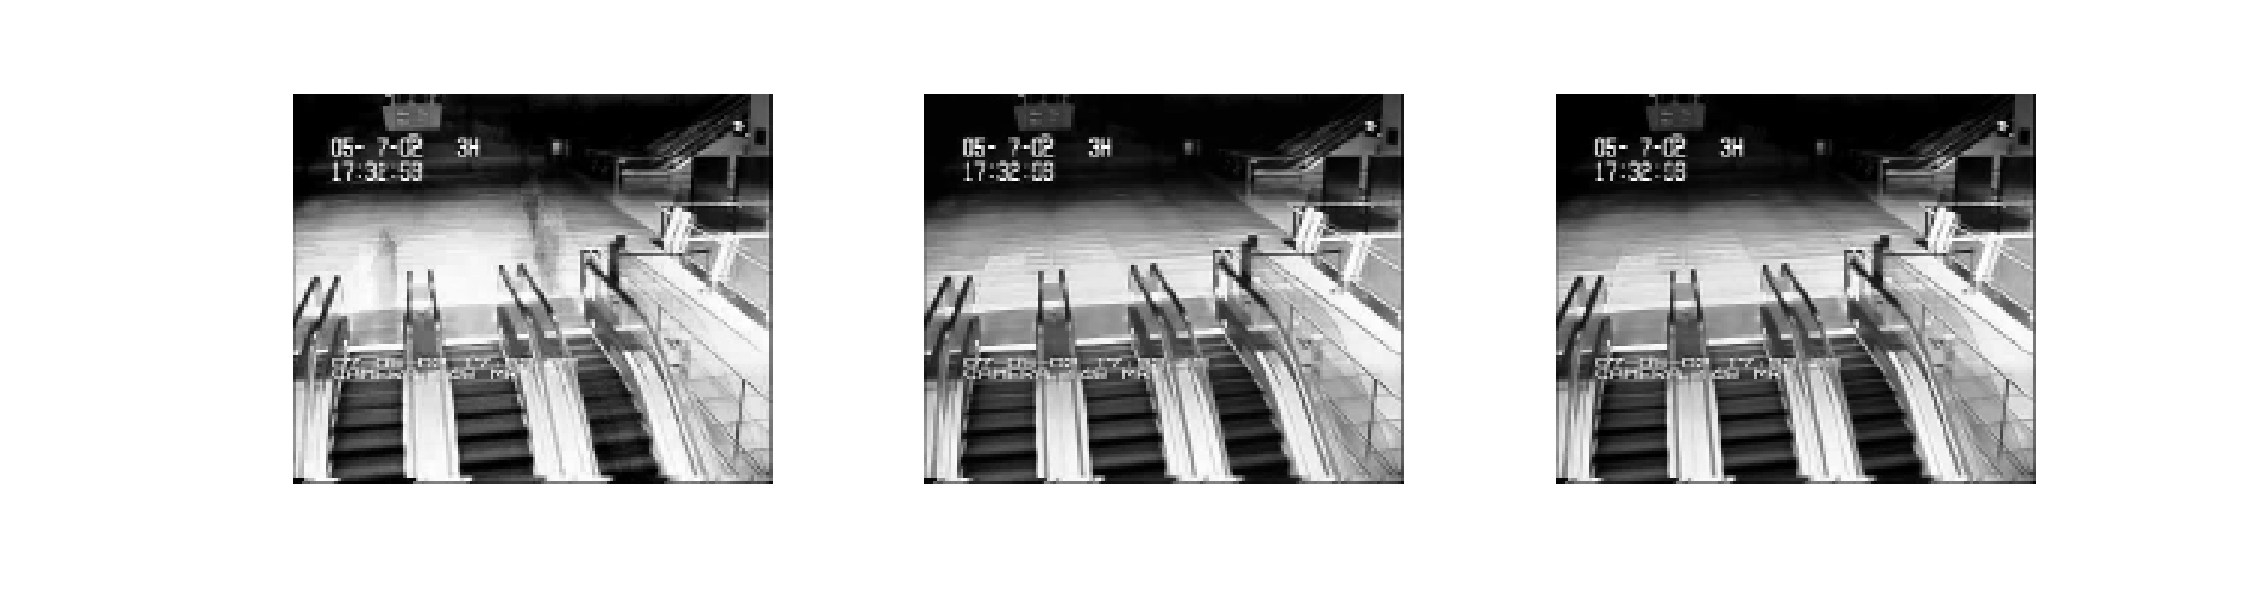
\includegraphics[width=6in]{L3slices_Penalty.pdf} }}%
   \\
   \subfloat[S3 Penalty]{{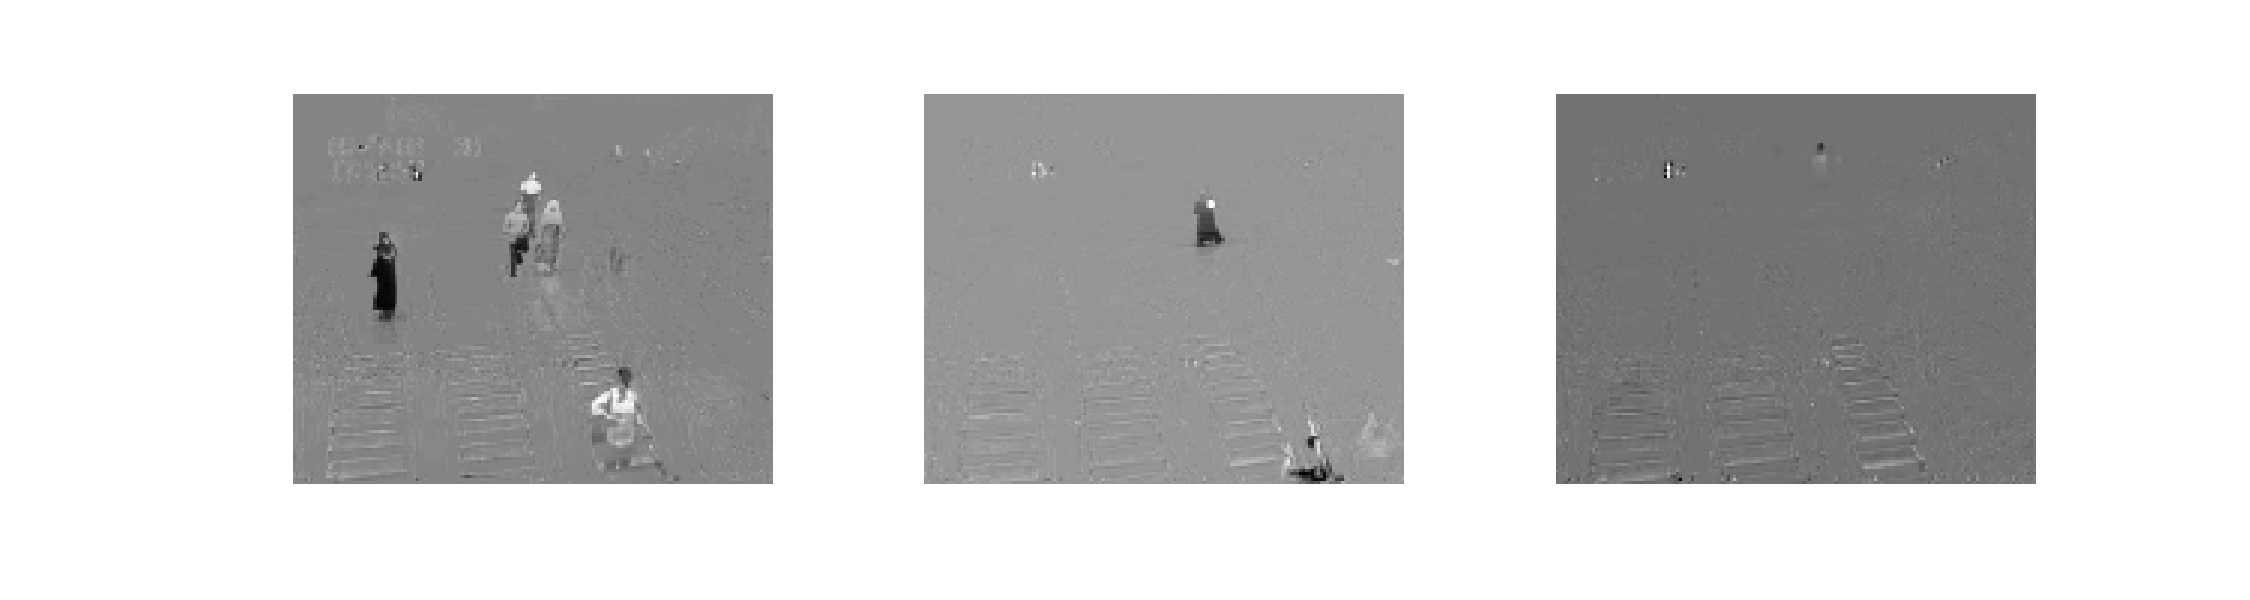
\includegraphics[width=6in]{S3slices_Penalty.pdf} }}%
   \\
\end{figure}
\newpage
\begin{figure}[H]%
   \centering
   \subfloat[Random Variable ADMM]{{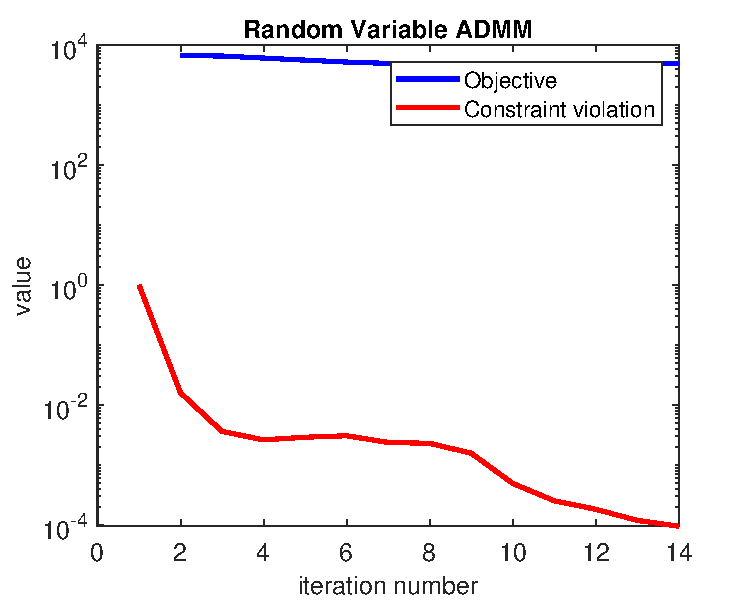
\includegraphics[width=3in]{RandomVariableADMM.pdf} }}%
   \subfloat[Random Variable Penalty]{{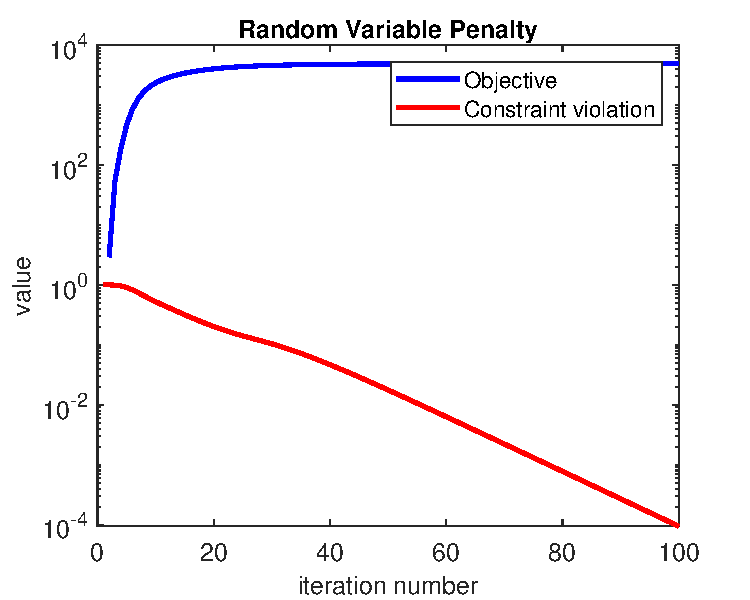
\includegraphics[width=3in]{RandomVariablePenalty.pdf} }}%
   \\
   \subfloat[Escalator ADMM]{{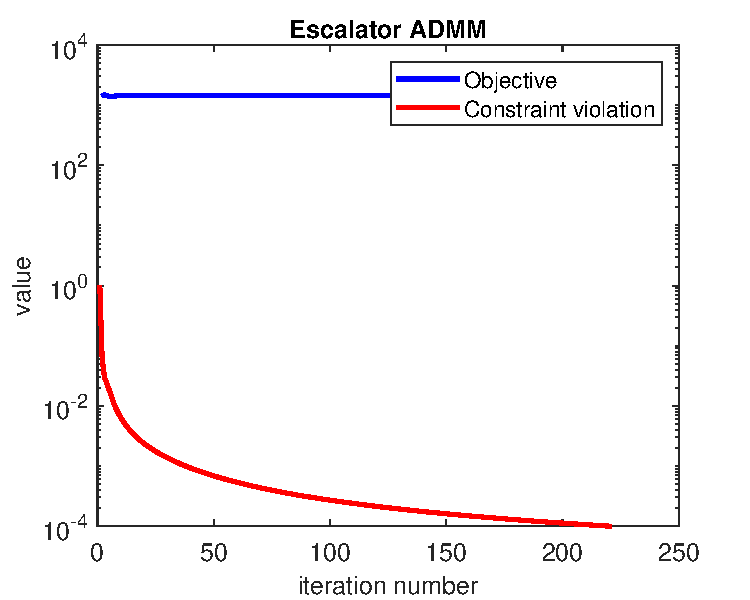
\includegraphics[width=3in]{Escalator ADMM.pdf} }}%
   \subfloat[Escalator Penalty]{{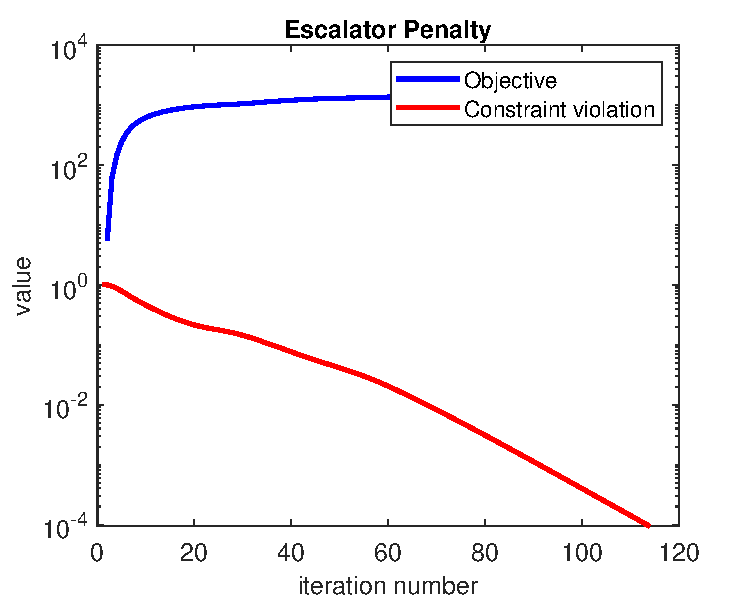
\includegraphics[width=3in]{EscalatorPenalty.pdf} }}%   
\end{figure}

\newpage
\textbf{Discussion}\\
Looking at the graphs for each of the four cases we see an obvious trend. For the quadratic penalty method, we can see a clear trend on how the objective value converges the more iterations we do. For both the random variable test and the escalator test we can see that objective value converges as we do more iterations. Since the y axis was plotted at a exponential scale, with ever index representing an order of 10 bigger. This means that it increases exponentially at first and then levels off. This makes sense because we added a penalty parameter to this particular problem. For the constraint violation, which is how much the dual feasibility has been violated, we can see a linear decrease in error on this scale. This means that as more iterations are being performed, we are constantly reducing the error for the dual feasibility on both tests. What is interesting is that even though the objective is outputting similar values the error is still decreasing on this scale.

For ADMM we see a different trend in our graphs. The objective value is near flat on both test cases. Since this scale is based on orders of 10, it implies that the objective might have increased but not as much for each specific case even though it converges. On the random variable test for ADMM the objective decreases and on the escalator the objective increases. This makes sense because unlike the penalty method, there was no penalty term which contributed to it's exponentially convergent behavior. As for the the constraint violation we see that for the two examples it's decreases look logarithmic on this scale. Meaning that error is near convergent on $1e^-4$ for both cases. For the random variable it appears that the there are iterations like 1 and 10, where the error decreases more drastically. 

Based on the console output of our code, our ADMM Solver performed better on the Random Data Sample and the Penalty Solver performed better on the escalator data. Because the results and final residual between both tests for both data samples are similar to each (percent error and image slices for random and escalator data, respectively), the performance of our algorithms are based off of the elapsed time and number of iterations. We expected that the ADMM Solver would be better in both cases, we think that the reason our ADMM algorithm was outperformed by the Penalty algorithm was due to lack of fine tuning of the variable $\mu$. When forming the Penalty method we spent a lot of time fine tuning the warm start and iteration updates so that it would terminate within reasonable time and with good results. We did not have the time to do the same for ADMM. In the ADMM algorithm we do not iteratively update $\mu$ which could have a negative affect on how efficiently our algorithm handles the subproblems. If we had more time, we would have continued optimizing the $\mu$ parameter. However, when plotting the constraint violations between each algorithm, the constraint violation of the ADMM algorithm initially converges at a must faster rate (see graphs). This supports our claim that the closed form solutions and iterative steps for ADMM are in fact more efficient and that fine tuning and further experimentation with parameters, such as $\mu$, would give us results that would reflect this. In the case of Robust PCA, we believe that ADMM is generally a better algorithm.
\newpage
\section*{References}
In addition to lecture notes and previous homework assignments:
\begin{itemize}
    \item Balandat, M., Krichene, W., Lam, C. and Lam, K., 2012. Robust Principal Component Analysis. [online] People.eecs.berkeley.edu.
    \item Cai, J., Candes, E. and Shen, Z., 2010. A singular value thresholding algorithm for matrix completion. SIAM Journal on optimization,.
    \item Lin, Z., Chen, M. and Ma, Y., 2011. The Augmented Lagrange Multiplier Method For Exact Recovery Of Corrupted Low-Rank Matrices. [online] Arxiv.org.
\end{itemize}

\end{document}
